\documentclass{standalone}
\usepackage{amsfonts, amsmath, amssymb, bm} %Math fonts and symbols
\usepackage{dcolumn, multirow} % decimal-aligned columns, multi-row cells
\usepackage[colorlinks=true]{hyperref}
\usepackage{graphicx, subfigure, float} % graphics commands
\usepackage[margin=1in]{geometry} % sets page layout
\usepackage{setspace}% allows toggling of double/single-spacing
\usepackage{verbatim}% defines environment for un-evaluated code
\usepackage{natbib}% defines citation commands and environments.
\singlespace % set document spacing to single
\bibpunct[, ]{(}{)}{,}{a}{}{,} % sets the punctuation of the bibliography entires.
\newcolumntype{d}[1]{D{.}{.}{#1}} % defines a decimal-aligned column
\usepackage{tikz}
\usetikzlibrary{intersections}
\usepackage{enumerate}
\usepackage[utf8]{inputenc}
\usepackage[english]{babel}
\hyphenpenalty=10000

\begin{document}
    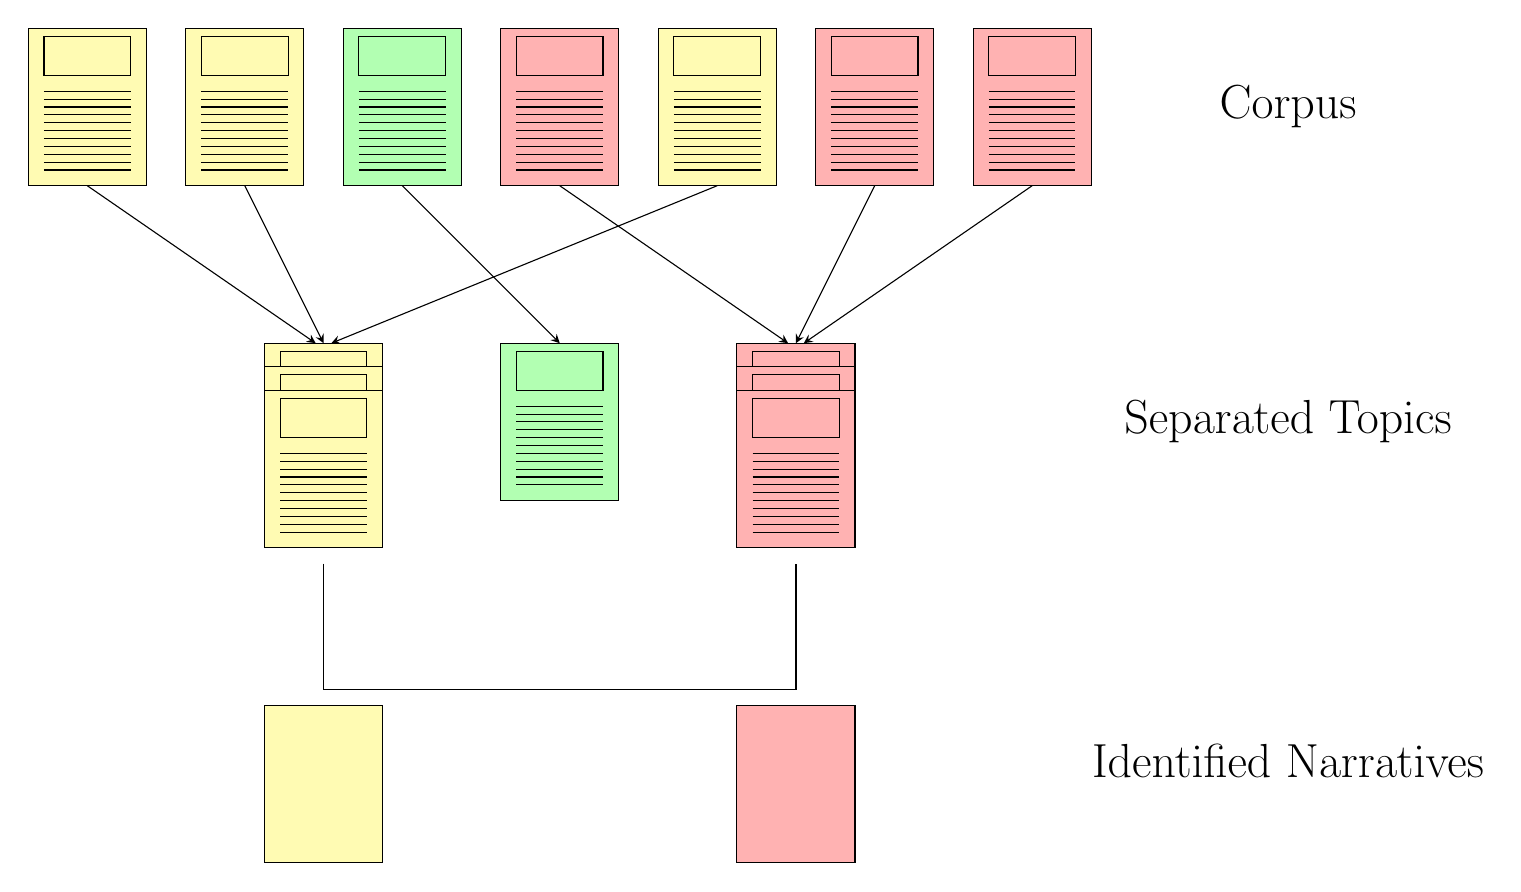
\begin{tikzpicture}[>=stealth, small/.style={
		% The shape:
		rectangle,
		% The size:
		minimum size=.75cm,
		% The border
		thick, draw=black,
		% The filling
		fill=white}]
    \foreach \x/\y in {0/0,2/0,8/0}{
      \draw [fill = yellow!30] (\x + 0,0 - \y) rectangle (\x + 1.5,2 - \y);
      \draw (\x + .2,1.4 - \y) rectangle (\x + 1.3,1.9 - \y);
      \foreach \z in {.2,.3,...,1.3}{
        \draw (\x + .2,\z - \y) -- (\x + 1.3,\z - \y);
      }
    }
    \foreach \x/\y in {12/0,6/0,10/0}{
      \draw [fill = red!30] (\x + 0,0 - \y) rectangle (\x + 1.5,2 - \y);
      \draw (\x + .2,1.4 - \y) rectangle (\x + 1.3,1.9 - \y);
      \foreach \z in {.2,.3,...,1.3}{
        \draw (\x + .2,\z - \y) -- (\x + 1.3,\z - \y);
      }
    }
    \foreach \x/\y in {4/0}{
      \draw [fill = green!30] (\x + 0,0 - \y) rectangle (\x + 1.5,2 - \y);
      \draw (\x + .2,1.4 - \y) rectangle (\x + 1.3,1.9 - \y);
      \foreach \z in {.2,.3,...,1.3}{
        \draw (\x + .2,\z - \y) -- (\x + 1.3,\z - \y);
      }
    }
    \foreach \x/\y in {3/4, 3/4.3, 3/4.6}{
      \draw [fill = yellow!30] (\x + 0,0 - \y) rectangle (\x + 1.5,2 - \y);
      \draw (\x + .2,1.4 - \y) rectangle (\x + 1.3,1.9 - \y);
      \foreach \z in {.2,.3,...,1.3}{
        \draw (\x + .2,\z - \y) -- (\x + 1.3,\z - \y);
      }
    }
    \foreach \x/\y in {9/4, 9/4.3, 9/4.6}{
      \draw [fill = red!30] (\x + 0,0 - \y) rectangle (\x + 1.5,2 - \y);
      \draw (\x + .2,1.4 - \y) rectangle (\x + 1.3,1.9 - \y);
      \foreach \z in {.2,.3,...,1.3}{
        \draw (\x + .2,\z - \y) -- (\x + 1.3,\z - \y);
      }
    }
    \foreach \x/\y in {6/4}{
      \draw [fill = green!30] (\x + 0,0 - \y) rectangle (\x + 1.5,2 - \y);
      \draw (\x + .2,1.4 - \y) rectangle (\x + 1.3,1.9 - \y);
      \foreach \z in {.2,.3,...,1.3}{
        \draw (\x + .2,\z - \y) -- (\x + 1.3,\z - \y);
      }
    }
    \draw (.75,0) [->] -- (3.65, -2);
    \draw (2.75,0) [->] -- (3.75, -2);
    \draw (8.75,0) [->] -- (3.85, -2);
    \draw (4.75,0) [->] -- (6.75, -2);
    \draw (6.75,0) [->] -- (9.65, -2);
    \draw (10.75,0) [->] -- (9.75, -2);
    \draw (12.75,0) [->] -- (9.85, -2);

    \draw [fill = yellow!30] (3, -8.6) rectangle (4.5, -6.6);
    \draw [fill = red!30] (9, -8.6) rectangle (10.5, -6.6);

    \draw (3.75, -4.8) -- ++(270:1.6) -- ++(0:6) -- ++(90:1.6);

    \node at (16,1) {\LARGE Corpus};
    \node at (16,-3) {\LARGE Separated Topics};
    \node at (16,-7.3) {\LARGE Identified Narratives};

    \end{tikzpicture}
\end{document}
